\documentclass[11pt]{article}

\usepackage[margin=1in]{geometry}
\usepackage{graphicx}
\usepackage{booktabs}
\usepackage{caption}
\usepackage{authblk}
\usepackage{lineno}
\usepackage[numbers,super,sort&compress]{natbib}
\usepackage{hyperref}
\usepackage{microtype}

\hypersetup{
  colorlinks=true,
  linkcolor=black,
  citecolor=black,
  urlcolor=black
}

\linenumbers

\title{\bfseries Background-matched evaluation reveals co-resistance background sensitivity in MALDI-TOF antimicrobial resistance prediction}

\author[1]{Byung Kim}
\author[2]{Yucheng Wang}
\author[3]{Nicolas Samuel Khoury-Levy}
\affil[1]{United States Air Force Academy, Colorado Springs, CO, USA}
\affil[2]{University of Wisconsin--Madison, Madison, WI, USA}
\affil[3]{Cornell University, Ithaca, NY, USA}
\date{}

\begin{document}
\maketitle

\begin{abstract}
Machine learning on MALDI-TOF mass spectra can predict antimicrobial resistance (AMR), but cross-site performance may reflect resistant-population background rather than focal resistance biology. Resistant isolates often co-segregate with clonal lineage, co-resistance blocks, mobile elements and site-specific ecology. We developed a model-agnostic background-matched audit that asks whether isolate-level predictions still distinguish resistant from susceptible isolates after matching on non-focal antimicrobial susceptibility testing (AST) labels. In an expanded \textit{E. coli} DRIAMS panel (four sites, six drugs), ciprofloxacin retained within-background signal at A-2018, DRIAMS-C and DRIAMS-D (background-centered AUC 0.703, 0.646 and 0.596), whereas amoxicillin-clavulanic acid weakened or collapsed toward chance (0.541, 0.497 and 0.486). A no-spectrum co-resistance-only baseline matched or exceeded the MALDI CNN for amoxicillin-clavulanic acid at external sites and outperformed MALDI for several cephalosporin rows, showing that AST background alone can explain substantial apparent performance. In a second-organism check, \textit{S. aureus}/oxacillin exceeded the co-resistance-only baseline and retained signal at A-2018 (centered AUC 0.763, 9 strata) and DRIAMS-C (0.699, 2 strata). A \textit{Klebsiella pneumoniae}/ceftriaxone extension showed the opposite behavior: raw AUC collapsed to chance after matching or became non-interpretable because no valid matched strata remained. Similar attenuation across CNN, multi-task LightGBM and single-task LightGBM outputs showed that background sensitivity was not architecture-specific. Cross-resistance networks identified near-perfect ciprofloxacin/norfloxacin coupling ($\phi=0.976$) and a strong cephalosporin block ($\phi=0.804$--0.884). In public WGS-linked UPEC data, MALDI peaks predicted ST131 lineage (AUC 0.932), and exact sequence-type centering attenuated ciprofloxacin and ceftriaxone AUCs to 0.564 and 0.503. Background-matched evaluation is a practical guardrail for interpreting MALDI-AMR models before deployment.
\end{abstract}

\section*{Introduction}

Antimicrobial resistance is a major global health burden, and delayed effective therapy worsens patient outcomes in severe bacterial infection\cite{amrCollaborators2022,kumar2006septicShock,seymour2017sepsis}. Clinical microbiology laboratories therefore need susceptibility information that is both rapid and reliable. MALDI-TOF mass spectrometry is already embedded in routine workflows for organism identification because it is inexpensive, high-throughput and compatible with clinical isolate processing\cite{croxatto2012maldiReview,vanbelkum2017maldiIssues,hou2019maldiStatus}. This installed infrastructure has motivated a growing body of work asking whether the same spectra can predict AMR directly, including broad DRIAMS benchmarking, topological and kernel methods, deep learning, multi-label learning and pathogen-specific studies\cite{weis2020topological,weis2020systematic,weis2022driams,wang2022vre,astudillo2024multilabel}.

The central unresolved issue is not whether MALDI-TOF AMR classifiers can produce non-trivial AUC values. Weis \textit{et al.} assembled more than 300,000 spectra and more than 750,000 linked AST phenotypes across four institutions, showing that calibrated MALDI models can reach clinically relevant cross-site performance for several organism-drug pairs\cite{weis2022driams,driamsdryad}. The harder question is what those predictions mean biologically. Routine MALDI-TOF spectra mostly capture abundant proteins in a low-mass range used for species identification. Those spectra can contain lineage-associated protein variation, site-associated sample-processing effects and ecological structure that are not the focal resistance mechanism. Thus, a classifier trained to separate resistant from susceptible isolates can in principle learn any spectral correlate of the resistant population, including clonal background, co-resistance burden or hospital-specific mixture, rather than the direct focal-drug mechanism.

This problem is familiar in bacterial genomics. Machine-learning AMR prediction from whole-genome data can be biased by population structure when resistant and susceptible labels are distributed unevenly across clonal lineages\cite{earle2016bacterialGwas,yu2025population}. The same logic applies to MALDI-TOF spectra: if the resistant isolates in a training set are concentrated in a spectrally recognizable lineage, the model can achieve high AUC by recognizing that lineage. This is not necessarily useless, because lineage-associated resistance can be clinically predictive in some settings. But it is fragile. A model that uses resistant-population background may fail when the same drug resistance is carried by different lineages, or when the local deployment population has a different mixture of clones, resistance plasmids and co-resistance patterns.

Existing clinical prediction reporting frameworks require transparent descriptions of development, validation, model inputs, missingness, calibration and performance\cite{tripod2015,probast2019,tripodAI2024}. TRIPOD+AI provides harmonized guidance for reporting regression and machine-learning prediction models\cite{tripodAI2024}, and PROBAST remains a widely used risk-of-bias framework for prediction-model studies\cite{probast2019}. These standards are necessary, but they do not specifically ask whether AMR predictions survive after controlling for co-resistance background. In the MALDI-AMR field, Weis \textit{et al.} proposed hierarchical stratification by spectral similarity to reduce over-optimistic estimates caused by close spectral neighbors in train and test sets\cite{weis2022stratification}. That approach is conceptually important, but it requires raw spectra or spectral distances and is tied to representation choices. It does not provide a simple post hoc audit that any laboratory can run from a prediction table alone.

Here we introduce a background-matched audit for MALDI-TOF AMR prediction. The audit is deliberately simple. For each focal drug, isolates are grouped by the AST labels of the other drugs in the same panel. The audit then asks whether the model still ranks focal-drug-resistant isolates above focal-drug-susceptible isolates inside those matched co-resistance backgrounds. This is a matched-analysis analogue for prediction-table auditing, drawing on the same principle that comparisons are more interpretable when made within covariate-defined strata\cite{rosenbaumRubin1983,austin2011propensity}. Unlike propensity-score matching, however, our goal is not causal estimation. The target is an operational question for clinical ML evaluation: how much of a MALDI-AMR model's apparent performance survives after the most obvious AST-background shortcut has been removed?

We apply the audit to an expanded \textit{E. coli} panel from DRIAMS and use \textit{E. coli}/ciprofloxacin versus \textit{E. coli}/amoxicillin-clavulanic acid as the primary contrast. Ciprofloxacin resistance in \textit{E. coli} is strongly associated with disseminated extraintestinal lineages, especially ST131, whereas amoxicillin-clavulanic acid resistance is more heterogeneous and can arise through multiple beta-lactamase, porin and regulatory contexts\cite{nicolas2014st131,price2013st131,benzakour2016st131,canton2011coresistance,pal2015cooccurrence}. We then add a focused \textit{S. aureus}/oxacillin generality check, because methicillin resistance is tied to \textit{mecA}/PBP2a and cell-wall remodeling and is expected to carry a different biological and ecological signal\cite{chambers1997mrsa}. Finally, we compare CNN, multi-task LightGBM, single-task LightGBM and published-workflow Weis logistic-regression outputs, and we use an independent WGS-linked UPEC cohort to test whether MALDI peak features can encode lineage strongly enough to plausibly drive AMR prediction.

\section*{Results}

\subsection*{Audit design: prediction-table matching on non-focal AST background}

The background-matched audit requires only a flat isolate-level prediction table: isolate identifier, site, year, organism, focal drug, binary AST label and model probability. For each focal drug, the audit constructs a background signature from the AST labels of all non-focal drugs in the same organism panel. For example, when ciprofloxacin is the focal drug in the \textit{E. coli} panel, the background signature records norfloxacin, amoxicillin-clavulanic acid, ceftriaxone, ceftazidime and cefepime labels. Isolates sharing a signature form a stratum. A stratum is considered valid only if it contains at least three resistant and three susceptible isolates for the focal drug.

The audit reports five quantities (Fig.~\ref{fig:framework}). Raw AUC is the ordinary unadjusted score over all isolates. Matched AUC recomputes AUC after retaining only isolates in valid strata. Background-centered AUC subtracts each stratum's mean model score and computes a pooled AUC from the residual scores. Pairwise within-background accuracy is the fraction of resistant-susceptible pairs within the same valid stratum for which the resistant isolate receives a higher score, with ties counted as 0.5. Matched retention reports how many focal-drug rows remain after exact background matching. Background-centered AUC is a higher-powered stratum-adjusted statistic, but pairwise accuracy is the direct within-stratum ranking test. We therefore treat a result as interpretable only when both the AUC estimate and matched support are adequate.

\begin{figure}[ht]
\centering
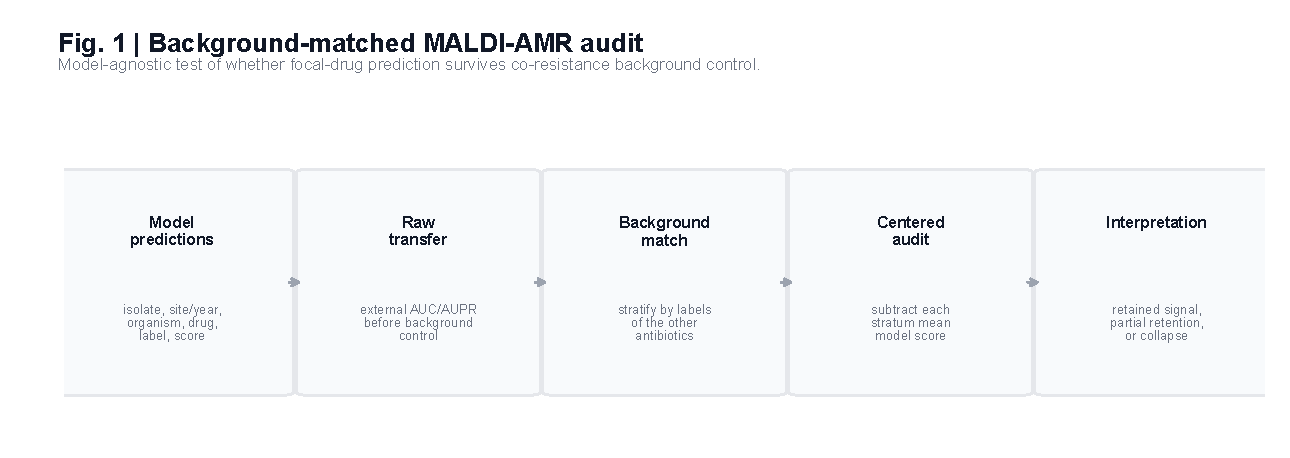
\includegraphics[width=\linewidth]{figures/figure_1_framework.pdf}
\caption{\textbf{Background-matched MALDI-AMR audit.} The audit accepts isolate-level prediction rows from any model. Non-focal AST labels define co-resistance background strata. Within each focal drug and site, valid strata contain at least three resistant and three susceptible isolates. The audit reports raw AUC, matched AUC, background-centered AUC, pairwise within-background accuracy and matched retention. The method is model-agnostic and can be applied retrospectively to any prediction table.}
\label{fig:framework}
\end{figure}

\subsection*{Co-resistance-only baselines reveal when AST background alone predicts the focal label}

We first asked how well the focal drug can be predicted without MALDI spectra. For each site and focal drug, a co-resistance-only baseline scored each isolate by the leave-one-out resistance prevalence of its exact non-focal AST background. This baseline is intentionally simple. If it performs well, the dataset contains a strong AST-label shortcut, and any MALDI model must exceed that baseline before its performance can be interpreted as added spectral value.

The baseline exposed several drug-site rows where AST background alone was highly predictive (Fig.~\ref{fig:three-way}). For extended-spectrum cephalosporins at DRIAMS-B and DRIAMS-C, co-resistance-only AUC reached 0.997--1.000. For norfloxacin at A-2018, co-resistance-only AUC was nearly perfect. These values are not surprising once the co-resistance network is inspected: ciprofloxacin and norfloxacin were almost collinear ($\phi=0.976$, resistant Jaccard 0.963), and ceftriaxone, ceftazidime and cefepime formed a strong cephalosporin block ($\phi=0.804$--0.884; Table~\ref{tab:cross-resistance}). In these settings, the non-focal AST pattern nearly determines the focal drug label.

The baseline also clarified the primary negative-control phenotype. For \textit{E. coli}/amoxicillin-clavulanic acid, the no-spectrum baseline matched or exceeded the CNN at all external sites: DRIAMS-B 0.796 versus 0.694, DRIAMS-C 0.687 versus 0.535 and DRIAMS-D 0.522 versus 0.557. Thus, at DRIAMS-B and DRIAMS-C, a trivial AST-background predictor was better than the MALDI model. At DRIAMS-D, both were close to chance. By contrast, \textit{E. coli}/ciprofloxacin at DRIAMS-D showed the largest MALDI-over-background margin in the expanded panel: CNN raw AUC 0.671 versus co-resistance-only AUC 0.522, with background-centered AUC 0.596. This made DRIAMS-D the most informative ciprofloxacin site because the model retained modest residual signal where AST background alone was weak.

\begin{figure}[ht]
\centering
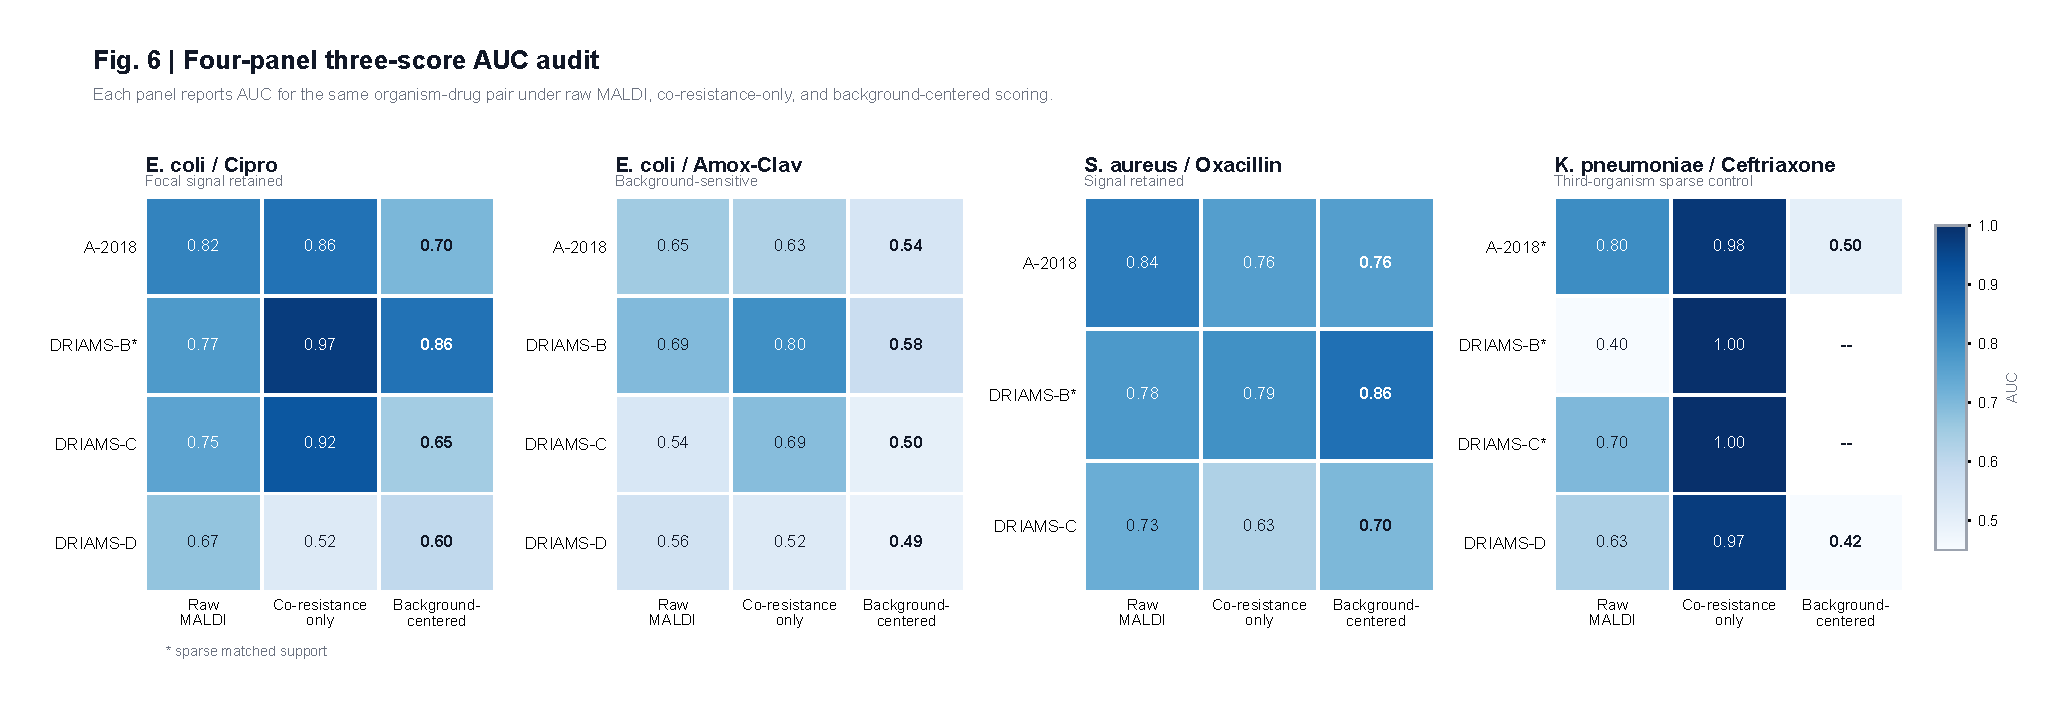
\includegraphics[width=\linewidth]{figures/figure_8_three_way_decomposition.pdf}
\caption{\textbf{Four-panel three-score decomposition of MALDI and AST-background signal.} Each panel is one organism-drug pair; within each panel, each cell reports raw MALDI AUC, no-spectrum co-resistance-only AUC or background-centered MALDI AUC for the same site. \textit{E. coli}/amoxicillin-clavulanic acid shows weak or chance-level centered AUC and a competitive co-resistance-only baseline at external sites. \textit{E. coli}/ciprofloxacin retains centered signal at interpretable sites, with the clearest MALDI-over-background margin at DRIAMS-D. \textit{S. aureus}/oxacillin shows retained signal at A-2018 and DRIAMS-C; DRIAMS-B has sparse matched support and is not treated as strong evidence.}
\label{fig:three-way}
\end{figure}

\input{tables/table_3_cross_resistance_edges.tex}

The norfloxacin rows illustrate why matched retention must be interpreted biologically. Because ciprofloxacin and norfloxacin were nearly perfectly coupled, norfloxacin-focal matching often placed ciprofloxacin status inside the background signature. A norfloxacin-resistant background therefore almost always implied ciprofloxacin resistance, leaving few or no strata with both norfloxacin-resistant and norfloxacin-susceptible isolates. Norfloxacin rows with zero valid strata are therefore not software failures; they are evidence that the fluoroquinolone pair is too collinear for exact-background focal-drug testing in this panel.

\subsection*{\textit{E. coli}/ciprofloxacin retained signal, whereas amoxicillin-clavulanic acid weakened or collapsed}

The primary background-matched contrast compared \textit{E. coli}/ciprofloxacin with \textit{E. coli}/amoxicillin-clavulanic acid across the same organism, sites, model family and audit procedure. Ciprofloxacin retained residual discrimination after background matching. Background-centered AUC was 0.703 at A-2018, 0.646 at DRIAMS-C and 0.596 at DRIAMS-D (Fig.~\ref{fig:primary-audit}; Table~\ref{tab:primary-audit}). Pairwise within-background accuracy was directionally consistent: 0.754 at A-2018, 0.675 at DRIAMS-C and 0.616 at DRIAMS-D. These values are attenuated relative to raw AUC, but they remain above chance in the main interpretable rows.

DRIAMS-B ciprofloxacin is reported but not used as primary evidence. Only one valid background stratum and 25 matched isolates were retained, producing a high centered estimate (0.860) with wide uncertainty. In a single stratum, matched and centered AUC can equal or exceed raw AUC because the retained stratum is a selected subset of the site and the stratum mean can shift residual ordering relative to the full population. That behavior is mathematically possible but statistically uninformative here; the low matched support is the reason for the caution flag.

Amoxicillin-clavulanic acid showed a different pattern. At DRIAMS-C and DRIAMS-D, background-centered AUC fell to 0.497 and 0.486, and pairwise within-background accuracy fell below chance (0.484 and 0.471). At A-2018 and DRIAMS-B, centered AUC was 0.541 and 0.576, indicating weak or borderline residual signal rather than robust focal-drug discrimination. The same table therefore contains both sides of the argument: ciprofloxacin retained attenuated but interpretable signal inside matched backgrounds, whereas amoxicillin-clavulanic acid was largely explained by background or collapsed toward chance.

\begin{figure}[ht]
\centering
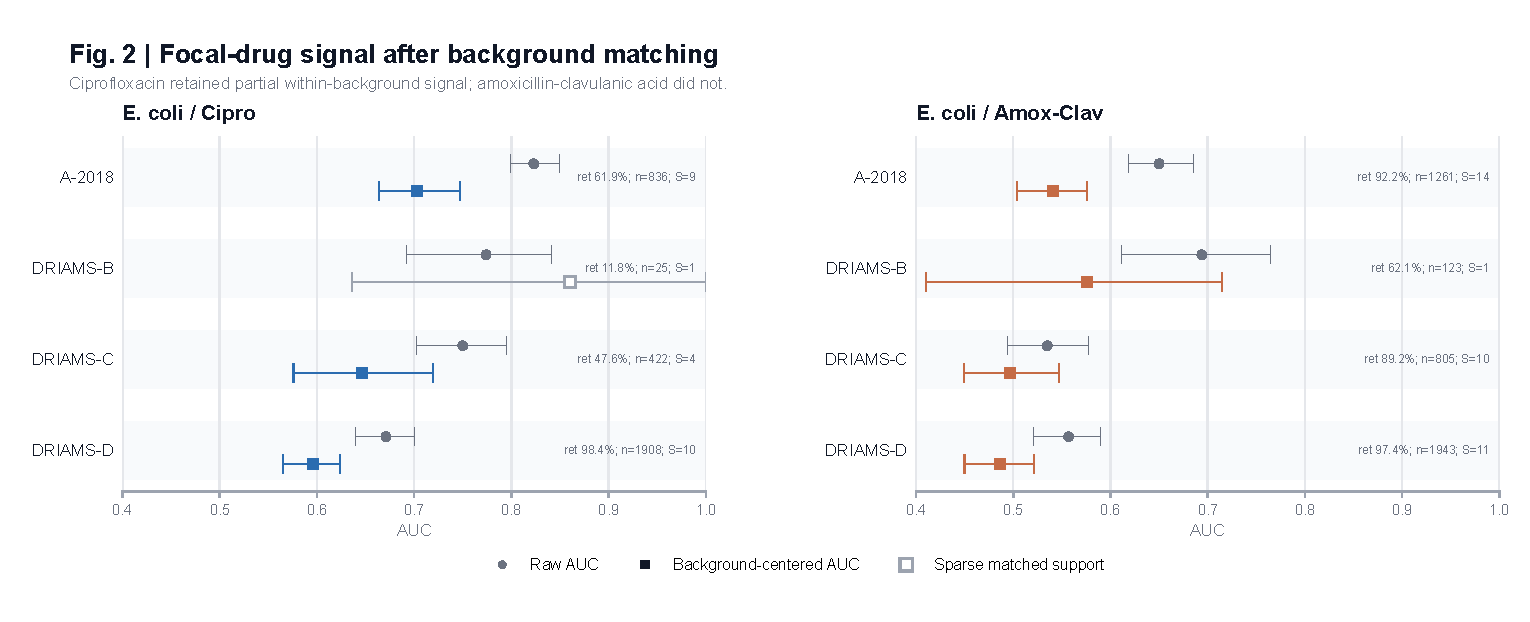
\includegraphics[width=\linewidth]{figures/figure_2_primary_background_audit.pdf}
\caption{\textbf{Primary \textit{E. coli} background-matched contrast.} Circles denote raw external AUC and squares denote background-centered AUC after co-resistance-stratum mean adjustment. Ciprofloxacin retains residual signal at the temporal site and two external sites. Amoxicillin-clavulanic acid weakens at A-2018 and DRIAMS-B and collapses toward chance at DRIAMS-C and DRIAMS-D. Error bars show 95\% bootstrap confidence intervals from 500 replicates.}
\label{fig:primary-audit}
\end{figure}

\input{tables/table_1_primary_audit.tex}

\subsection*{Falsification controls show that background burden can outperform MALDI for beta-lactam rows}

To test whether the audit was merely rediscovering raw AUC attenuation, we added two falsification controls. First, a background-burden score counted non-focal resistant drugs and asked whether a simple resistance-burden number could predict the focal label. Second, a within-background label shuffle preserved background strata while disrupting focal-label association.

The background-burden control was competitive with or stronger than the MALDI model for several beta-lactam rows. At A-2018, background-burden AUC exceeded observed MALDI AUC for cefepime (0.985 versus 0.867), ceftazidime (0.938 versus 0.838) and ceftriaxone (0.874 versus 0.863). At DRIAMS-C, the same pattern was stronger: cefepime 0.931 versus 0.648, ceftazidime 0.945 versus 0.609 and ceftriaxone 0.934 versus 0.623. These controls make the negative result more useful, not less. They show that some impressive raw MALDI AUCs are achievable by counting co-resistant drugs and therefore should not be interpreted as evidence of focal spectral biology without background-matched retention.

For ciprofloxacin, the burden score was also competitive at A-2018 and DRIAMS-C, but the within-background shuffle control showed that the observed model score exceeded the shuffled null at A-2018, DRIAMS-C and DRIAMS-D. This is consistent with the main audit: ciprofloxacin contains both background structure and residual signal, whereas several beta-lactam rows are dominated by co-resistance ecology.

\subsection*{\textit{S. aureus}/oxacillin provides a second-organism generality check, not broad validation}

We next applied the same audit to a \textit{S. aureus}/oxacillin panel. This is a useful second-organism check because oxacillin resistance is linked to methicillin resistance and \textit{mecA}/PBP2a biology, rather than the \textit{E. coli} fluoroquinolone or beta-lactam ecologies considered above\cite{chambers1997mrsa}. The result supported generality of the framework while also showing why cautious adequacy labels matter.

The CNN/Mega model exceeded the co-resistance-only baseline at A-2018 (raw AUC 0.838 versus baseline 0.762; background-centered AUC 0.763 across 9 valid strata) and DRIAMS-C (raw AUC 0.725 versus baseline 0.627; background-centered AUC 0.699 across 2 valid strata). Pairwise within-background accuracy was also above chance at A-2018 (0.770) and DRIAMS-C (0.719). DRIAMS-B produced a high centered estimate (0.864), but only one valid stratum was available; we therefore treat it as sparse support rather than strong evidence. DRIAMS-D is absent from this export because the oxacillin label was not available in the exported \textit{S. aureus} panel at that site, so no DRIAMS-D conclusion is made.

\subsection*{Background sensitivity replicates across model classes}

To test whether the audit result was specific to the CNN, we repeated the analysis for multi-task LightGBM and single-task LightGBM prediction exports. The same qualitative pattern held (Fig.~\ref{fig:model-family}; Table~\ref{tab:model-replication}). \textit{E. coli}/ciprofloxacin retained background-centered signal across CNN, multi-task LightGBM and single-task LightGBM at A-2018 and DRIAMS-C, with partial or weak retention at DRIAMS-D. \textit{E. coli}/amoxicillin-clavulanic acid weakened or collapsed across all three model classes. \textit{S. aureus}/oxacillin retained signal for CNN/Mega and both LightGBM variants at A-2018 and DRIAMS-C, while DRIAMS-B remained sparse.

\begin{figure}[ht]
\centering
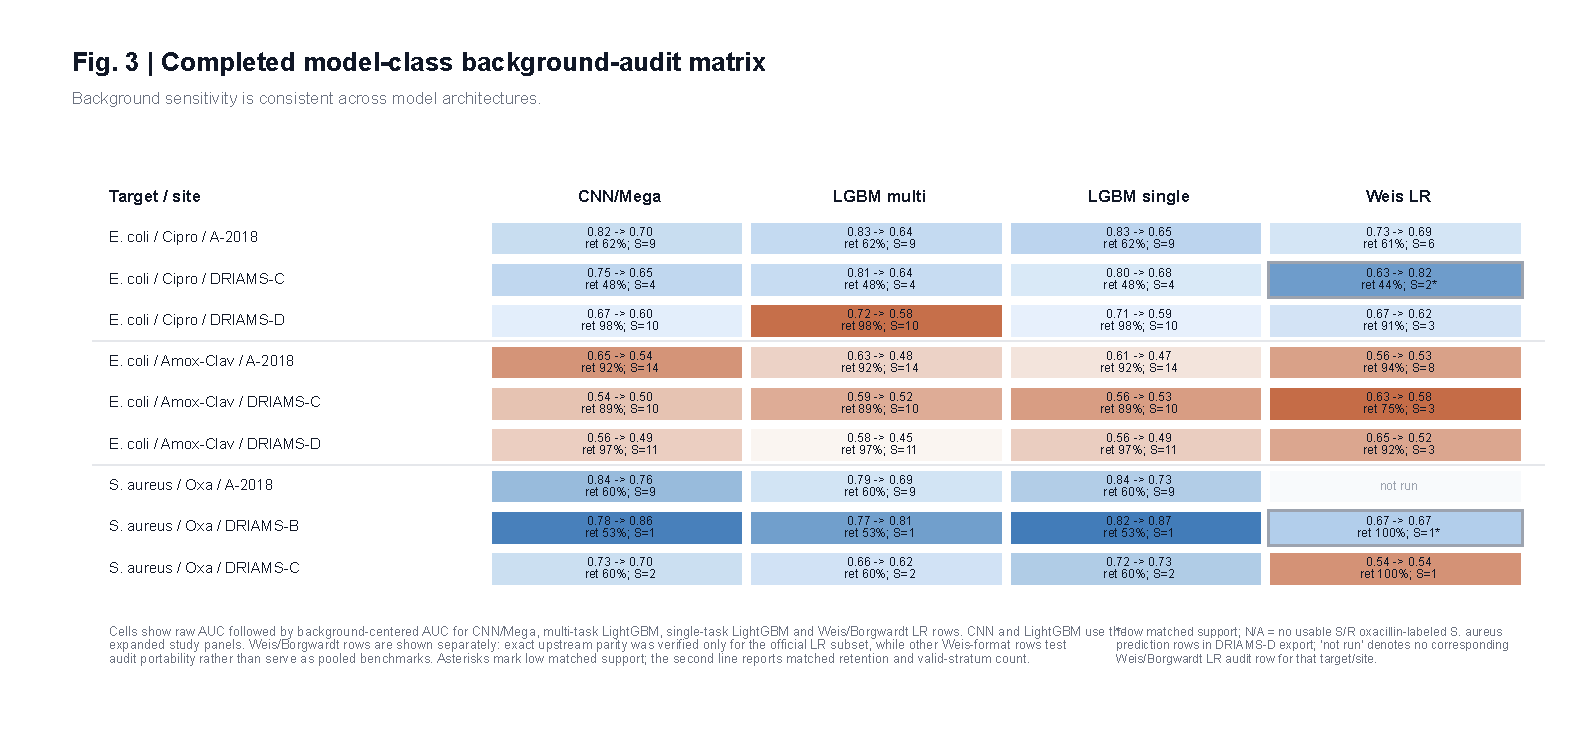
\includegraphics[width=\linewidth]{figures/figure_3_model_family_replication.pdf}
\caption{\textbf{Background sensitivity is consistent across model architectures.} Cells show raw AUC followed by background-centered AUC for CNN/Mega, multi-task LightGBM, single-task LightGBM and Weis/Borgwardt LR rows. CNN and LightGBM use the expanded study panels. Weis/Borgwardt rows are shown separately: exact upstream parity was verified only for the official LR subset, while other Weis-format rows test audit portability rather than serve as pooled benchmarks. Asterisks mark low matched support; retention and valid-stratum counts are reported in the source data.}
\label{fig:model-family}
\end{figure}

\begin{table}[ht]
\centering
\scriptsize
\caption{Raw and background-centered AUCs across model families for the primary E. coli contrast.}
\label{tab:model-replication}
\resizebox{\linewidth}{!}{%
\begin{tabular}{llrrrrrrrrl}
\toprule
Site & Drug & CNN/Mega raw & CNN/Mega centered & LGBM multi raw & LGBM multi centered & LGBM single raw & LGBM single centered & Weis LR raw & Weis LR centered & Consensus \\
\midrule
A-2018 & Cipro & 0.823 & 0.703 & 0.828 & 0.640 & 0.828 & 0.652 & 0.734 & 0.689 & retained \\
DRIAMS-C & Cipro & 0.750 & 0.646 & 0.814 & 0.637 & 0.804 & 0.682 & 0.625 & 0.816* & retained \\
DRIAMS-D & Cipro & 0.671 & 0.596 & 0.723 & 0.576 & 0.712 & 0.591 & 0.667 & 0.620 & partial \\
A-2018 & Amox-Clav & 0.650 & 0.541 & 0.635 & 0.482 & 0.614 & 0.465 & 0.564 & 0.529 & weak \\
DRIAMS-C & Amox-Clav & 0.535 & 0.497 & 0.593 & 0.518 & 0.559 & 0.533 & 0.626 & 0.578 & collapsed \\
DRIAMS-D & Amox-Clav & 0.557 & 0.486 & 0.580 & 0.449 & 0.559 & 0.487 & 0.652 & 0.524 & collapsed \\
\bottomrule
\end{tabular}%
}
\vspace{2mm}\parbox{0.95\linewidth}{\footnotesize Columns separate raw and background-centered AUCs for direct model-family comparison. Asterisks mark caution rows with low matched support. Weis LR cells combine the temporal A-2018 export with existing Weis-style DRIAMS-C/DRIAMS-D compatibility rows; they are compatibility evidence rather than pooled benchmarks with the CNN/LightGBM panel.}
\end{table}


The Weis logistic-regression compatibility rows are intentionally interpreted separately. They use the published-workflow panel and demonstrate that the audit can be applied to Weis-style prediction exports, but they are not symmetric with the expanded \textit{E. coli} CNN/LGBM panel. For \textit{S. aureus}/oxacillin, the Weis LR DRIAMS-C row is weak (AUC 0.543), whereas the CNN/Mega \textit{S. aureus} panel retains stronger centered signal. These are different prediction exports and should not be pooled.

The same atlas-style workflow also adds a representative \textit{Klebsiella pneumoniae}/ceftriaxone extension and summarizes all currently available prediction sets (Tables~\ref{tab:organism-extension} and \ref{tab:audit-atlas-summary}). Together with \textit{S. aureus}/oxacillin, these rows test whether the finding is only an \textit{E. coli}/ciprofloxacin story. The \textit{S. aureus} rows provide a second-organism retained-signal case, whereas \textit{Klebsiella}/ceftriaxone provides a third-organism background-sensitive or sparse-control case. Full \textit{Klebsiella} six-drug results are reported in the Supplementary Information.

\begin{table}[ht]
\centering
\scriptsize
\caption{Representative organism-extension audit rows.}
\label{tab:organism-extension}
\resizebox{\linewidth}{!}{%
\begin{tabular}{lllrrrrll}
\toprule
Organism/drug & Model & Site & Raw AUC & Centered AUC & Background AUC & Retention (\%) & Strata & Interpretation \\
\midrule
S. aureus / Oxacillin & CNN/Mega & A-2018 & 0.838 & 0.763 & 0.762 & 60.1 & 9 & strong within background signal \\
S. aureus / Oxacillin & CNN/Mega & DRIAMS-B & 0.775 & 0.864 & 0.795 & 52.6 & 1 & background only competitive but residual signal \\
S. aureus / Oxacillin & CNN/Mega & DRIAMS-C & 0.725 & 0.699 & 0.627 & 59.6 & 2 & moderate within background signal \\
S. aureus / Oxacillin & Weis LR & DRIAMS-B & 0.667 & 0.667 & -- & 100.0 & 1 & caution low matched support \\
S. aureus / Oxacillin & Weis LR & DRIAMS-C & 0.543 & 0.543 & -- & 100.0 & 1 & weak raw signal \\
K. pneumoniae / Ceftriaxone & CNN/Mega & A-2018 & 0.804 & 0.500 & 0.981 & 3.3 & 1 & background only competitive and weak residual \\
K. pneumoniae / Ceftriaxone & CNN/Mega & DRIAMS-B & 0.404 & -- & 1.000 & 0.0 & 0 & not interpretable or sparse \\
K. pneumoniae / Ceftriaxone & CNN/Mega & DRIAMS-C & 0.698 & -- & 1.000 & 0.0 & 0 & not interpretable or sparse \\
K. pneumoniae / Ceftriaxone & CNN/Mega & DRIAMS-D & 0.630 & 0.424 & 0.973 & 81.8 & 2 & background only competitive and weak residual \\
K. pneumoniae / Ceftriaxone & Weis LR & DRIAMS-B & 0.509 & 0.509 & -- & 100.0 & 1 & near chance or ambiguous \\
K. pneumoniae / Ceftriaxone & Weis LR & DRIAMS-C & 0.672 & 0.672 & -- & 100.0 & 1 & cautionary moderate within background signal \\
K. pneumoniae / Ceftriaxone & Weis LR & DRIAMS-D & 0.596 & 0.596 & -- & 100.0 & 1 & weak or partial within background signal \\
\bottomrule
\end{tabular}%
}
\vspace{2mm}\parbox{0.95\linewidth}{\footnotesize Representative rows test whether the audit is only an E. coli/ciprofloxacin story. S. aureus/oxacillin is a second-organism retained-signal case; K. pneumoniae/ceftriaxone is a third-organism background-sensitive or sparse-control case. Weis LR rows are compatibility exports; background-only AUC was not computed for those rows.}
\end{table}


\begin{table}[ht]
\centering
\scriptsize
\caption{Audit atlas coverage and outcome summary.}
\label{tab:audit-atlas-summary}
\resizebox{\linewidth}{!}{%
\begin{tabular}{lllrrrrrr}
\toprule
Atlas set & Model & Scope & Rows & Drugs & Sites & Interpretable & Retained/partial & Background-sensitive \\
\midrule
ecoli\_cnn & CNN/Mega & E. coli six-drug panel & 23 & 6 & 4 & 18 & 8 & 9 \\
ecoli\_lgbm\_multi & LightGBM multi-task & E. coli six-drug panel & 23 & 6 & 4 & 18 & 7 & 10 \\
ecoli\_lgbm\_single & LightGBM single-task & E. coli six-drug panel & 23 & 6 & 4 & 18 & 6 & 11 \\
weis\_lr\_ecoli\_temporal\_a2018 & Weis LR & E. coli six-drug temporal A-2018 panel & 6 & 6 & 1 & 4 & 2 & 2 \\
saureus\_cnn & CNN/Mega & S. aureus oxacillin panel & 25 & 7 & 4 & 23 & 12 & 7 \\
saureus\_lgbm\_multi & LightGBM multi-task & S. aureus oxacillin panel & 25 & 7 & 4 & 23 & 13 & 7 \\
saureus\_lgbm\_single & LightGBM single-task & S. aureus oxacillin panel & 25 & 7 & 4 & 23 & 14 & 8 \\
klebsiella\_cnn & CNN/Mega & K. pneumoniae six-drug panel & 24 & 6 & 4 & 15 & 4 & 11 \\
weis\_lr\_klebsiella\_ceftriaxone & Weis LR & K. pneumoniae ceftriaxone official-panel extension & 3 & 1 & 3 & 3 & 2 & 0 \\
weis\_lr\_ecoli & Weis LR & E. coli Weis-style panel & 17 & 6 & 3 & 9 & 4 & 5 \\
\bottomrule
\end{tabular}%
}
\vspace{2mm}\parbox{0.95\linewidth}{\footnotesize The atlas combines background-matched audit rows, exact-background baselines, calibration checks and sensitivity summaries. Retained/partial counts include rows classified as retained or partial residual signal by the atlas rules.}
\end{table}


\begin{figure}[ht]
\centering
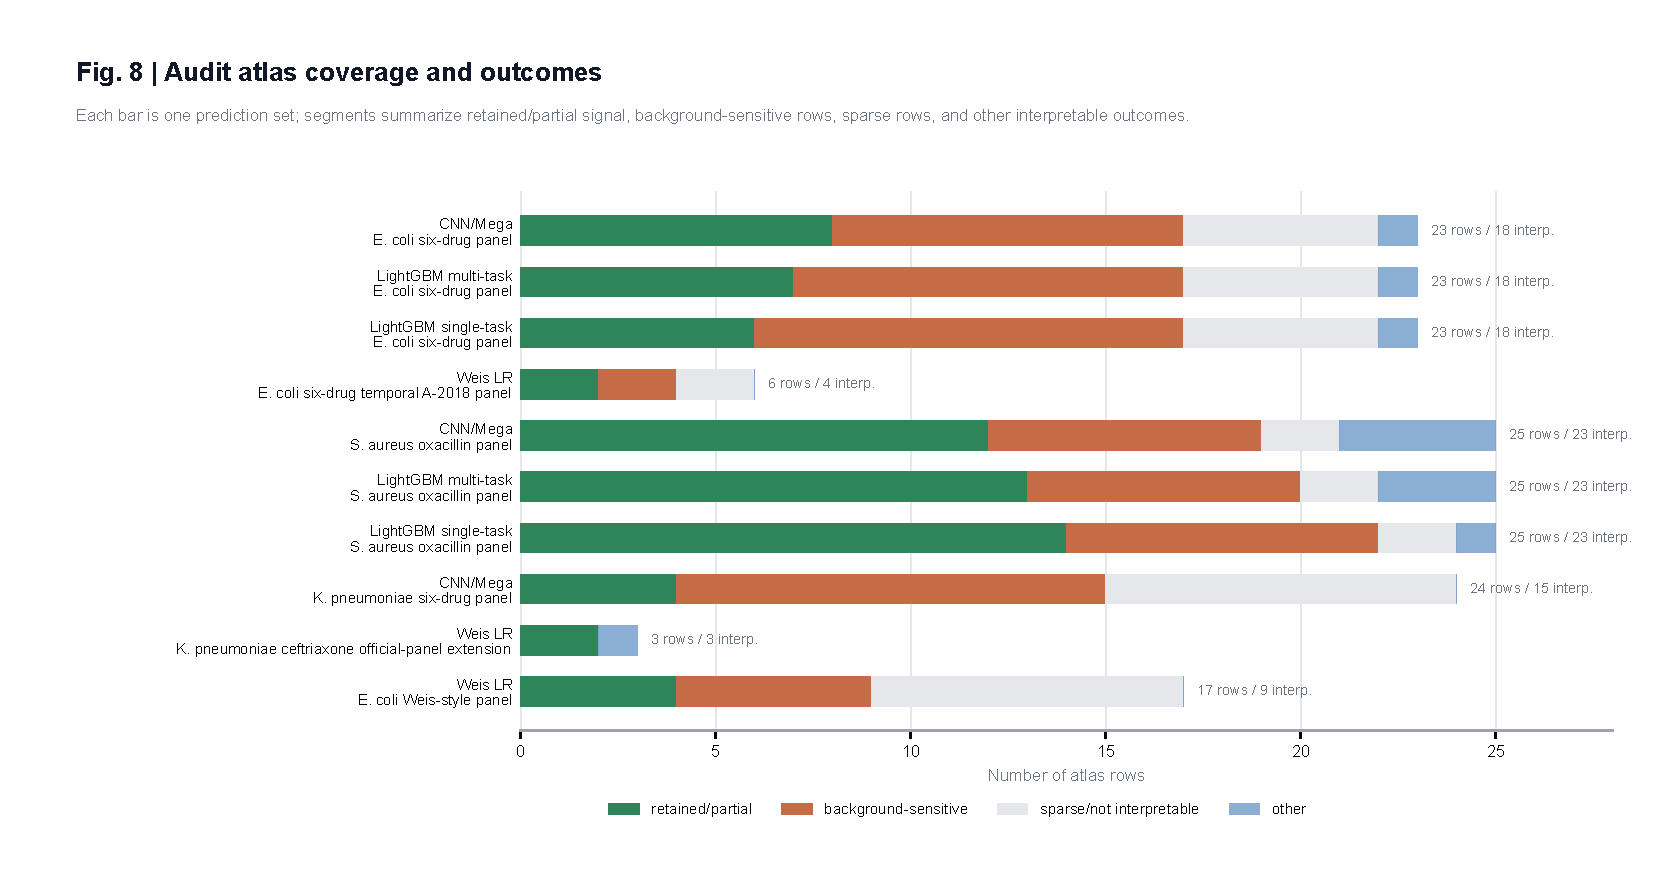
\includegraphics[width=\linewidth]{figures/figure_11_audit_atlas_summary.pdf}
\caption{\textbf{Audit atlas coverage and outcomes.} Each bar summarizes one prediction set in the current atlas. Segments show retained or partial residual signal, background-sensitive rows, sparse or non-interpretable rows and other interpretable outcomes.}
\label{fig:audit-atlas-summary}
\end{figure}

\subsection*{Public WGS-linked UPEC data support the biological plausibility of lineage-mediated MALDI signal}

The DRIAMS audit uses co-resistance background because WGS labels are not available for the primary DRIAMS isolates. To ask whether lineage is actually visible in MALDI features, we analyzed an independent public Basel uropathogenic \textit{E. coli} cohort with WGS metadata and Bruker MALDI-derived peak features\cite{cuenod2023papgii}. A simple centroid-direction classifier predicted ST131 lineage from MALDI peaks with AUC 0.932 (407 isolates, 55 ST131), substantially higher than ciprofloxacin resistance (AUC 0.755) or ceftriaxone resistance (AUC 0.689) in the same cohort (Fig.~\ref{fig:public-wgs}; Table~\ref{tab:public-wgs}).

\begin{figure}[ht]
\centering
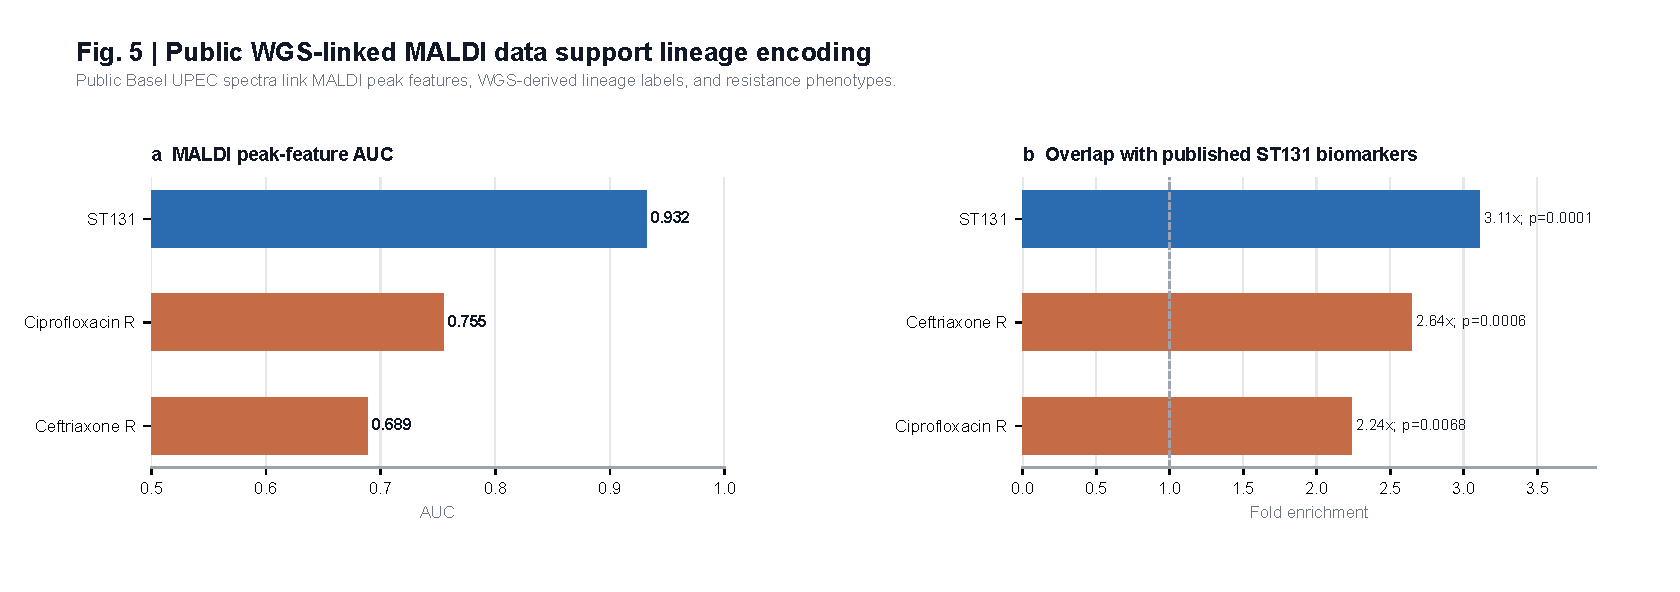
\includegraphics[width=\linewidth]{figures/figure_5_public_wgs_proteomic_support.pdf}
\caption{\textbf{Independent WGS-linked UPEC support for lineage-associated MALDI signal.} MALDI peak features predicted ST131 lineage more strongly than ciprofloxacin or ceftriaxone resistance in a public WGS-linked UPEC cohort. Exact sequence-type centering attenuated resistance AUCs, and discriminative bins were enriched near published ST131 MALDI biomarker masses. These analyses provide biological support for the audit interpretation but do not replace WGS-linked validation in DRIAMS.}
\label{fig:public-wgs}
\end{figure}

Sequence-type control attenuated resistance prediction. Exact-ST centering reduced ciprofloxacin AUC from 0.755 to 0.564 among retained sequence types containing both resistant and susceptible isolates, and reduced ceftriaxone AUC from 0.689 to 0.503. In ST131-only isolates, ceftriaxone resistance was near chance (AUC 0.515), while ciprofloxacin remained partially predictable (AUC 0.725). These results do not prove that the DRIAMS-trained model uses ST131, because the UPEC cohort is independent. They do show that routine MALDI peak features can encode lineage strongly enough for lineage to become a plausible shortcut in AMR prediction.

\input{tables/table_4_public_wgs_auc.tex}

\input{tables/table_6_upec_clone_control.tex}

We also tested whether resistance-discriminative MALDI bins overlapped published ST131 biomarker mass neighborhoods\cite{nakamura2019st131}. Among the top 75 discriminative bins for each target, ST131, ciprofloxacin and ceftriaxone all showed enrichment near published ST131 marker masses (permutation $P=0.0001$, 0.0068 and 0.0006, respectively). This is a mass-neighborhood enrichment test, not protein identification; nevertheless, it supports the claim that lineage-associated spectral regions and resistance-associated discriminative regions can overlap.

\section*{Discussion}

This study makes a specific claim: MALDI-TOF AMR prediction is sensitive to resistant-population background, and that sensitivity can be quantified from prediction tables alone. It does not claim that all MALDI-AMR models are invalid, that resistance prediction is impossible, or that every high AUC is caused by clonal confounding. The key finding is more practical. Raw cross-site AUC is not enough to distinguish focal-drug signal from co-resistance background. A model can look useful in aggregate while failing to rank resistant isolates above susceptible isolates inside matched AST backgrounds.

The clearest example is the \textit{E. coli} primary contrast. Ciprofloxacin retained attenuated signal inside matched backgrounds, whereas amoxicillin-clavulanic acid weakened or collapsed. This difference is biologically coherent. Fluoroquinolone-resistant \textit{E. coli}, especially ST131-associated resistance, can present a stable lineage-linked proteomic signature across sites\cite{nicolas2014st131,price2013st131,benzakour2016st131,nakamura2019st131}. Amoxicillin-clavulanic acid resistance is more heterogeneous, can involve multiple beta-lactamase and permeability contexts, and may not map to a stable focal spectral pattern\cite{canton2011coresistance,pal2015cooccurrence}. The audit does not directly identify the mechanism. It shows that the prediction survives background matching for one phenotype and not the other.

The co-resistance-only baseline is central to the interpretation. It converts a qualitative concern--that models may exploit co-resistance ecology--into a direct benchmark. If a no-spectrum baseline using only non-focal AST labels matches or exceeds the MALDI model, raw MALDI performance cannot be taken as evidence of spectral focal-drug biology. This result was strongest for cephalosporins and amoxicillin-clavulanic acid at external sites. In those settings, the model was often no better than, and sometimes worse than, simple background burden or exact-background prevalence. That does not make the result uninteresting. It identifies organism-drug-site combinations where the dataset itself contains enough co-resistance structure to inflate ordinary performance.

The \textit{S. aureus}/oxacillin analysis is important because it moves the framework beyond a single \textit{E. coli}/ciprofloxacin story. Oxacillin retained signal at A-2018 and DRIAMS-C and exceeded the co-resistance-only baseline at both sites. However, this should be framed as a second-organism generality check, not as a full atlas. DRIAMS-B had only one valid matched stratum, and DRIAMS-D was absent from the export. The correct conclusion is that the audit can identify retained signal outside \textit{E. coli}, and that \textit{S. aureus}/oxacillin is a promising retained-signal case, while systematic organism-drug coverage remains future work.

Our framework is complementary to Weis hierarchical stratification rather than redundant with it\cite{weis2022stratification}. Hierarchical stratification controls spectral similarity during train-test splitting and requires access to spectra or spectral distances. The present audit controls co-resistance background after prediction and requires only a prediction table plus non-focal AST labels. These answer different questions. Spectral stratification asks whether performance survives when close spectral neighbors are prevented from leaking across evaluation splits. Background matching asks whether a fixed model can still discriminate focal resistance inside the same co-resistance context. A strong MALDI-AMR evaluation should eventually report both, especially when raw AUC is intended to support clinical deployment.

The same logic also extends clinical ML reporting frameworks. TRIPOD+AI and PROBAST require transparent reporting, model-validation clarity and bias assessment\cite{probast2019,tripodAI2024}. They do not, however, specify a field-specific audit for AMR co-resistance structure. We propose background-matched AUC, pairwise within-background accuracy, matched retention and a co-resistance-only baseline as MALDI-AMR-specific additions to standard reporting. This is not a replacement for calibration, decision-curve analysis, external validation, data provenance or prospective clinical studies. It is a targeted guardrail for a known biological failure mode in microbial prediction.

Several limitations are important. First, AST background is an imperfect proxy for lineage. Isolates can share a co-resistance profile while belonging to different sequence types, and isolates from the same lineage can differ in plasmid content or resistance mechanism. WGS-linked DRIAMS data would be the strongest direct test. Second, background-centered AUC is a pooled stratum-adjusted statistic. It removes stratum-level mean score shifts but still computes a pooled AUC over residuals. This is why pairwise within-background accuracy and matched retention must always be reported. Third, exact matching can become impossible when non-focal and focal labels are nearly collinear, as in the ciprofloxacin/norfloxacin pair. Zero valid strata in that setting are biologically meaningful but not interpretable for focal-signal estimation. Fourth, the public UPEC WGS analysis is independent of DRIAMS and supports plausibility rather than direct causal attribution. Fifth, the biomarker overlap analysis is mass-neighborhood enrichment, not protein identification. Clinical linear-mode MALDI peak matching cannot establish protein identity without orthogonal proteomics.

The next major step is an audit atlas across many organism-drug pairs. A realistic atlas would not require WGS for every row. It would screen DRIAMS organism-drug-site combinations for matched retention, background-centered AUC, pairwise accuracy, co-resistance-only AUC and calibration. Only a subset would be interpretable, but the uninterpretable rows are themselves informative because they reveal where co-resistance structure is too strong for exact-background testing. A second major upgrade would be WGS or MLST linkage for a small, high-value subset: \textit{E. coli}/ciprofloxacin to test ST131, \textit{S. aureus}/oxacillin to test MRSA/MSSA lineage, and a beta-lactam row where co-resistance-only performance dominates.

The practical recommendation is straightforward. MALDI-TOF AMR studies should report raw AUC, calibration, external-site performance and standard clinical ML documentation, but they should also report a background-matched audit whenever multi-drug AST labels are available. A deployable model should demonstrate not only that it separates resistant from susceptible isolates in aggregate, but that it does so among isolates with the same non-focal AST background. The audit released here makes that check reproducible, model-agnostic and accessible to laboratories that can export isolate-level predictions.

\section*{Online Methods}

\subsection*{Primary DRIAMS benchmark}

We used DRIAMS MALDI-TOF spectra and AST labels as the primary clinical benchmark\cite{weis2022driams,driamsdryad}. Models were trained on DRIAMS-A isolates collected before 2018 and evaluated on a temporal DRIAMS-A 2018 hold-out plus external sites DRIAMS-B, DRIAMS-C and DRIAMS-D. External-site labels were not used for training, hyperparameter selection or calibration. Intermediate AST calls and rows with missing focal-drug labels were excluded from the relevant drug-level evaluation.

The expanded \textit{E. coli} panel comprised ciprofloxacin, norfloxacin, amoxicillin-clavulanic acid, ceftriaxone, ceftazidime and cefepime. The \textit{S. aureus}/oxacillin panel used oxacillin as the focal drug and penicillin, ciprofloxacin, erythromycin, clindamycin, gentamicin and fusidic acid as non-focal background drugs. The \textit{S. aureus} DRIAMS-D oxacillin row was not present in the prediction export and was therefore not analyzed.

\subsection*{CNN/Mega model}

The primary neural model was a multi-task one-dimensional CNN trained on 6,000-bin MALDI spectra spanning the 2,000--20,000 m/z range. The encoder used a 1D convolutional stem (32 channels, kernel size 15, stride 2), batch normalization, ReLU activation and max pooling, followed by three residual squeeze-and-excitation blocks with 64, 128 and 256 channels. Each residual block used two kernel-size-7 convolutions and a skip connection; channel attention was implemented with an adaptive average pooling squeeze-and-excitation module. Encoded spectra were globally average pooled to a 256-dimensional representation and passed through dropout (0.3).

Task conditioning used feature-wise linear modulation (FiLM) by organism-drug task identifier. The default architecture used one binary resistance head per active task and selected the head corresponding to the isolate's task. Domain-adversarial training used a gradient-reversal domain classifier over site labels, with the adversarial weight annealed up to 0.3. Resistance heads were trained with binary cross-entropy with logits and label smoothing of 0.05. Training used AdamW with learning rate $1\times10^{-4}$, weight decay $1\times10^{-4}$, cosine annealing, batch size 64, intraclass mixup ($\alpha=0.2$), early stopping by validation macro-AUC and five random seeds.

The encoder was initialized with masked autoencoder pretraining. The autoencoder masked 75\% of 50-bin patches and reconstructed masked spectral bins with mean-squared error loss. MAE pretraining used AdamW with learning rate $1\times10^{-3}$ for 30 epochs. The trained MAE stem and residual layers initialized the supervised CNN. These architectural details are reported because deployment-facing ML papers should document model form, optimization, loss functions and validation procedures rather than only citing a code repository\cite{tripodAI2024,probast2019}.

\subsection*{LightGBM and Weis logistic-regression comparisons}

LightGBM baselines were trained from the same spectral representation and train/test split as the CNN exports. We evaluated both multi-task and single-task LightGBM variants. These baselines were included to test whether background sensitivity was architecture-specific; they were not tuned to maximize benchmark performance.

Published-workflow Weis logistic-regression compatibility rows were exported using the official-panel workflow and then audited with the same background-matched script. These rows include \textit{E. coli}/ceftriaxone, \textit{Klebsiella pneumoniae}/ceftriaxone and \textit{S. aureus}/oxacillin. Because the published panel differs from the expanded \textit{E. coli} audit panel, these rows are labeled compatibility evidence rather than pooled with the CNN/LGBM primary contrast.

\subsection*{Background signatures and valid strata}

For every focal organism-drug-site row, we constructed a background signature by concatenating the non-focal drug AST calls for the same organism panel. Labels were represented as R, S or U when unavailable. Exact background signatures define strata. A stratum was valid if it contained at least three resistant and three susceptible isolates for the focal drug. Sensitivity analyses repeated the audit at stricter thresholds ($n\geq5$ and $n\geq10$ per class per stratum) and are reported in the repository outputs.

\subsection*{Audit metrics}

Raw AUC was computed from all available focal-drug prediction rows. Matched AUC was computed after restricting to isolates in valid background strata. Background-centered AUC subtracted each valid stratum's mean model score from each isolate score and then computed a pooled AUC over the residuals. Pairwise within-background accuracy enumerated all resistant-susceptible pairs within each valid stratum and counted the fraction in which the resistant isolate had the higher score. Ties were counted as 0.5. Matched retention was the proportion of focal-drug rows retained after exact background matching. Adequacy labels were assigned from valid-stratum count, matched sample size and retention; caution rows were shown but not used as primary evidence.

\subsection*{Co-resistance-only baseline and falsification controls}

The co-resistance-only baseline ignored spectra. For each isolate in background stratum $g$, with $r_g$ resistant isolates and $n_g$ total isolates, the leave-one-out smoothed score was
\[
  \frac{r_g-y_i+\alpha/2}{n_g-1+\alpha},
\]
where $y_i$ is the focal binary label and $\alpha=2$. This prevents the isolate's own label from determining its score. The resulting AUC measures how well exact non-focal AST background predicts the focal label. The background-burden falsification score counted the number of non-focal resistant labels. Within-background label-shuffle controls permuted focal labels within valid strata and recomputed AUC to estimate a null distribution preserving background structure.

\subsection*{Cross-resistance network}

For every pair of drugs in the \textit{E. coli} panel, we computed phi correlation, resistant-resistant lift and resistant Jaccard similarity using isolates with non-missing labels for both drugs. Phi correlation identifies label coupling; resistant Jaccard quantifies overlap among resistant isolates; resistant-resistant lift compares observed double resistance with the expected rate under independence.

\subsection*{Public WGS-linked UPEC validation}

We used public Basel/Cu\'{e}nod uropathogenic \textit{E. coli} resources linking WGS metadata and Bruker MALDI-derived peak features\cite{cuenod2023papgii}. After manifest joining, 407 isolates had complete Bruker peak features and usable WGS-derived sequence type metadata; 55 were ST131. Bruker peak features were binned into 50 Da intervals. A centroid-direction classifier was evaluated with five cross-validation folds for ST131 identity, ciprofloxacin resistance and ceftriaxone resistance. The classifier was intentionally simple so that the analysis tested whether the signal was present in the features rather than whether a complex model could be tuned.

Lineage-controlled resistance analyses repeated classification within ST131 and non-ST131 subsets and computed centered AUC after subtracting group-level mean scores for WGS-derived backgrounds. Backgrounds were ST131 status, exact sequence type and broad phylogroup. Exact sequence-type control retained only sequence types containing both resistant and susceptible isolates for the focal drug, so retained sample fractions are reported.

\subsection*{Published ST131 biomarker enrichment}

Published ST131 MALDI biomarker masses were taken from Nakamura \textit{et al.}\cite{nakamura2019st131}. For each target, we ranked bins by absolute class-mean log-intensity difference and selected the top 75 bins. Overlap with the biomarker list was assessed using a 40 Da window around each published mass and compared with a mass-stratified permutation null (1,000 permutations) that preserved the coarse m/z distribution of selected bins. This analysis tests non-random mass-neighborhood enrichment. It does not identify proteins, because clinical linear-mode whole-cell MALDI peak matching is not sufficient for confident protein assignment.

\subsection*{Software and reproducibility}

All analyses operate on a flat, model-agnostic prediction table with columns for isolate identifier, site, year, organism, drug, binary AST label and model probability. The audit engine is implemented in \texttt{run\_background\_audit\_framework.py}. Prediction exporters, atlas scripts and model-class matrix scripts are provided in \texttt{scripts/}. Publication figures and \LaTeX\ tables are created by \texttt{scripts/make\_ncomms\_figures.py}. Source-data CSV files for manuscript figures are in \texttt{manuscript/source\_data/}. The expected input schema is documented in \texttt{SCHEMA.md}; non-focal AST labels can be supplied either as long-form rows or as a precomputed background signature.

\section*{Data availability}

Raw DRIAMS spectra and AST files are available from the DRIAMS Dryad release\cite{driamsdryad} and are not redistributed here. Public UPEC WGS metadata and Bruker peak resources are available through the Cu\'{e}nod UPEC resources described in the original study\cite{cuenod2023papgii}. Processed summary outputs, derived tables and source-data CSV files for all manuscript figures are provided in the repository.

\section*{Code availability}

All analysis code is available at \url{https://github.com/byungkim113/background-matched-maldi-amr-audit}, including the audit engine, prediction exporters, co-resistance-only baseline, model-class matrix pipeline, public UPEC analyses, figure-generation code and reproducibility documentation.

\section*{Acknowledgements}

We thank the DRIAMS investigators and the Cu\'{e}nod UPEC investigators for releasing resources that make background-aware reanalysis possible.

\section*{Author contributions}

B.K. and Y.W. contributed equally as primary drivers of the project. B.K. and Y.W. jointly developed the study concept, background-matched audit framework, validation strategy, result interpretation and manuscript. B.K. led implementation of the audit pipeline, model-output analyses and figure generation. Y.W. led methodological framing, robustness/audit design, interpretation of biological and clinical implications and manuscript development. N.S.K.-L. contributed to study framing, result interpretation and critical manuscript revision. All authors reviewed and approved the manuscript.

\section*{Competing interests}

The authors declare no competing interests.

\section*{Additional information}

Correspondence and requests for materials should be addressed to B.K.

\bibliographystyle{unsrtnat}
\bibliography{references}

\end{document}
